% Options for packages loaded elsewhere
\PassOptionsToPackage{unicode}{hyperref}
\PassOptionsToPackage{hyphens}{url}
%
\documentclass[
]{article}
\usepackage{lmodern}
\usepackage{amssymb,amsmath}
\usepackage{ifxetex,ifluatex}
\ifnum 0\ifxetex 1\fi\ifluatex 1\fi=0 % if pdftex
  \usepackage[T1]{fontenc}
  \usepackage[utf8]{inputenc}
  \usepackage{textcomp} % provide euro and other symbols
\else % if luatex or xetex
  \usepackage{unicode-math}
  \defaultfontfeatures{Scale=MatchLowercase}
  \defaultfontfeatures[\rmfamily]{Ligatures=TeX,Scale=1}
\fi
% Use upquote if available, for straight quotes in verbatim environments
\IfFileExists{upquote.sty}{\usepackage{upquote}}{}
\IfFileExists{microtype.sty}{% use microtype if available
  \usepackage[]{microtype}
  \UseMicrotypeSet[protrusion]{basicmath} % disable protrusion for tt fonts
}{}
\makeatletter
\@ifundefined{KOMAClassName}{% if non-KOMA class
  \IfFileExists{parskip.sty}{%
    \usepackage{parskip}
  }{% else
    \setlength{\parindent}{0pt}
    \setlength{\parskip}{6pt plus 2pt minus 1pt}}
}{% if KOMA class
  \KOMAoptions{parskip=half}}
\makeatother
\usepackage{xcolor}
\IfFileExists{xurl.sty}{\usepackage{xurl}}{} % add URL line breaks if available
\IfFileExists{bookmark.sty}{\usepackage{bookmark}}{\usepackage{hyperref}}
\hypersetup{
  pdftitle={Topic 2: Exercise 1},
  pdfauthor={Daniel Alonso},
  hidelinks,
  pdfcreator={LaTeX via pandoc}}
\urlstyle{same} % disable monospaced font for URLs
\usepackage[margin=1in]{geometry}
\usepackage{color}
\usepackage{fancyvrb}
\newcommand{\VerbBar}{|}
\newcommand{\VERB}{\Verb[commandchars=\\\{\}]}
\DefineVerbatimEnvironment{Highlighting}{Verbatim}{commandchars=\\\{\}}
% Add ',fontsize=\small' for more characters per line
\usepackage{framed}
\definecolor{shadecolor}{RGB}{248,248,248}
\newenvironment{Shaded}{\begin{snugshade}}{\end{snugshade}}
\newcommand{\AlertTok}[1]{\textcolor[rgb]{0.94,0.16,0.16}{#1}}
\newcommand{\AnnotationTok}[1]{\textcolor[rgb]{0.56,0.35,0.01}{\textbf{\textit{#1}}}}
\newcommand{\AttributeTok}[1]{\textcolor[rgb]{0.77,0.63,0.00}{#1}}
\newcommand{\BaseNTok}[1]{\textcolor[rgb]{0.00,0.00,0.81}{#1}}
\newcommand{\BuiltInTok}[1]{#1}
\newcommand{\CharTok}[1]{\textcolor[rgb]{0.31,0.60,0.02}{#1}}
\newcommand{\CommentTok}[1]{\textcolor[rgb]{0.56,0.35,0.01}{\textit{#1}}}
\newcommand{\CommentVarTok}[1]{\textcolor[rgb]{0.56,0.35,0.01}{\textbf{\textit{#1}}}}
\newcommand{\ConstantTok}[1]{\textcolor[rgb]{0.00,0.00,0.00}{#1}}
\newcommand{\ControlFlowTok}[1]{\textcolor[rgb]{0.13,0.29,0.53}{\textbf{#1}}}
\newcommand{\DataTypeTok}[1]{\textcolor[rgb]{0.13,0.29,0.53}{#1}}
\newcommand{\DecValTok}[1]{\textcolor[rgb]{0.00,0.00,0.81}{#1}}
\newcommand{\DocumentationTok}[1]{\textcolor[rgb]{0.56,0.35,0.01}{\textbf{\textit{#1}}}}
\newcommand{\ErrorTok}[1]{\textcolor[rgb]{0.64,0.00,0.00}{\textbf{#1}}}
\newcommand{\ExtensionTok}[1]{#1}
\newcommand{\FloatTok}[1]{\textcolor[rgb]{0.00,0.00,0.81}{#1}}
\newcommand{\FunctionTok}[1]{\textcolor[rgb]{0.00,0.00,0.00}{#1}}
\newcommand{\ImportTok}[1]{#1}
\newcommand{\InformationTok}[1]{\textcolor[rgb]{0.56,0.35,0.01}{\textbf{\textit{#1}}}}
\newcommand{\KeywordTok}[1]{\textcolor[rgb]{0.13,0.29,0.53}{\textbf{#1}}}
\newcommand{\NormalTok}[1]{#1}
\newcommand{\OperatorTok}[1]{\textcolor[rgb]{0.81,0.36,0.00}{\textbf{#1}}}
\newcommand{\OtherTok}[1]{\textcolor[rgb]{0.56,0.35,0.01}{#1}}
\newcommand{\PreprocessorTok}[1]{\textcolor[rgb]{0.56,0.35,0.01}{\textit{#1}}}
\newcommand{\RegionMarkerTok}[1]{#1}
\newcommand{\SpecialCharTok}[1]{\textcolor[rgb]{0.00,0.00,0.00}{#1}}
\newcommand{\SpecialStringTok}[1]{\textcolor[rgb]{0.31,0.60,0.02}{#1}}
\newcommand{\StringTok}[1]{\textcolor[rgb]{0.31,0.60,0.02}{#1}}
\newcommand{\VariableTok}[1]{\textcolor[rgb]{0.00,0.00,0.00}{#1}}
\newcommand{\VerbatimStringTok}[1]{\textcolor[rgb]{0.31,0.60,0.02}{#1}}
\newcommand{\WarningTok}[1]{\textcolor[rgb]{0.56,0.35,0.01}{\textbf{\textit{#1}}}}
\usepackage{graphicx}
\makeatletter
\def\maxwidth{\ifdim\Gin@nat@width>\linewidth\linewidth\else\Gin@nat@width\fi}
\def\maxheight{\ifdim\Gin@nat@height>\textheight\textheight\else\Gin@nat@height\fi}
\makeatother
% Scale images if necessary, so that they will not overflow the page
% margins by default, and it is still possible to overwrite the defaults
% using explicit options in \includegraphics[width, height, ...]{}
\setkeys{Gin}{width=\maxwidth,height=\maxheight,keepaspectratio}
% Set default figure placement to htbp
\makeatletter
\def\fps@figure{htbp}
\makeatother
\setlength{\emergencystretch}{3em} % prevent overfull lines
\providecommand{\tightlist}{%
  \setlength{\itemsep}{0pt}\setlength{\parskip}{0pt}}
\setcounter{secnumdepth}{-\maxdimen} % remove section numbering
\ifluatex
  \usepackage{selnolig}  % disable illegal ligatures
\fi

\title{Topic 2: Exercise 1}
\author{Daniel Alonso}
\date{November 28th, 2020}

\begin{document}
\maketitle

\hypertarget{importing-libraries}{%
\paragraph{Importing libraries}\label{importing-libraries}}

\begin{Shaded}
\begin{Highlighting}[]
\FunctionTok{library}\NormalTok{(dplyr)}
\FunctionTok{library}\NormalTok{(Rcpp)}
\end{Highlighting}
\end{Shaded}

\hypertarget{importing-data-as-described-by-exercise}{%
\paragraph{Importing data as described by
exercise}\label{importing-data-as-described-by-exercise}}

\begin{Shaded}
\begin{Highlighting}[]
\NormalTok{d }\OtherTok{\textless{}{-}} \FunctionTok{read.csv}\NormalTok{(}\StringTok{"../../datasets/Colleges.csv"}\NormalTok{)}
\end{Highlighting}
\end{Shaded}

\hypertarget{replacing-binary-variable-private-with-1-and-0}{%
\paragraph{Replacing binary variable Private with 1 and
0}\label{replacing-binary-variable-private-with-1-and-0}}

\begin{Shaded}
\begin{Highlighting}[]
\NormalTok{d}\SpecialCharTok{$}\NormalTok{Private }\OtherTok{\textless{}{-}} \FunctionTok{ifelse}\NormalTok{(d}\SpecialCharTok{$}\NormalTok{Private }\SpecialCharTok{==} \StringTok{"Yes"}\NormalTok{, }\DecValTok{1}\NormalTok{, }\DecValTok{0}\NormalTok{)}
\end{Highlighting}
\end{Shaded}

\hypertarget{selecting-columns}{%
\paragraph{Selecting columns}\label{selecting-columns}}

\begin{Shaded}
\begin{Highlighting}[]
\NormalTok{data }\OtherTok{\textless{}{-}}\NormalTok{ d }\SpecialCharTok{\%\textgreater{}\%}\NormalTok{ dplyr}\SpecialCharTok{::}\FunctionTok{select}\NormalTok{(}\StringTok{\textquotesingle{}Private\textquotesingle{}}\NormalTok{,}\StringTok{\textquotesingle{}Apps\textquotesingle{}}\NormalTok{,}\StringTok{\textquotesingle{}Accept\textquotesingle{}}\NormalTok{,}\StringTok{\textquotesingle{}Enroll\textquotesingle{}}\NormalTok{,}\StringTok{\textquotesingle{}F.Undergrad\textquotesingle{}}\NormalTok{)}
\end{Highlighting}
\end{Shaded}

\hypertarget{calculating-covariances}{%
\paragraph{Calculating covariances}\label{calculating-covariances}}

\begin{Shaded}
\begin{Highlighting}[]
\NormalTok{cov\_matrix }\OtherTok{\textless{}{-}} \FunctionTok{cov}\NormalTok{(data)}
\NormalTok{cov\_matrix}
\CommentTok{\#\textgreater{}                   Private          Apps        Accept       Enroll  F.Undergrad}
\CommentTok{\#\textgreater{} Private         0.1986559     {-}745.3552     {-}519.2042    {-}235.1942    {-}1330.764}
\CommentTok{\#\textgreater{} Apps         {-}745.3552439 14978459.5301  8949859.8119 3045255.9876 15289702.474}
\CommentTok{\#\textgreater{} Accept       {-}519.2042169  8949859.8119  6007959.6988 2076267.7627 10393582.435}
\CommentTok{\#\textgreater{} Enroll       {-}235.1942393  3045255.9876  2076267.7627  863368.3923  4347529.884}
\CommentTok{\#\textgreater{} F.Undergrad {-}1330.7637175 15289702.4742 10393582.4355 4347529.8841 23526579.326}
\end{Highlighting}
\end{Shaded}

\newpage

\hypertarget{calculating-correlations}{%
\paragraph{Calculating correlations}\label{calculating-correlations}}

\begin{Shaded}
\begin{Highlighting}[]
\NormalTok{corr\_matrix }\OtherTok{\textless{}{-}} \FunctionTok{cov2cor}\NormalTok{(cov\_matrix)}
\NormalTok{corr\_matrix}
\CommentTok{\#\textgreater{}                Private       Apps     Accept     Enroll F.Undergrad}
\CommentTok{\#\textgreater{} Private      1.0000000 {-}0.4320947 {-}0.4752520 {-}0.5679078  {-}0.6155605}
\CommentTok{\#\textgreater{} Apps        {-}0.4320947  1.0000000  0.9434506  0.8468221   0.8144906}
\CommentTok{\#\textgreater{} Accept      {-}0.4752520  0.9434506  1.0000000  0.9116367   0.8742233}
\CommentTok{\#\textgreater{} Enroll      {-}0.5679078  0.8468221  0.9116367  1.0000000   0.9646397}
\CommentTok{\#\textgreater{} F.Undergrad {-}0.6155605  0.8144906  0.8742233  0.9646397   1.0000000}
\end{Highlighting}
\end{Shaded}

\hypertarget{experimenting-a-little-bit-with-the-private-variable}{%
\paragraph{Experimenting a little bit with the private
variable}\label{experimenting-a-little-bit-with-the-private-variable}}

Let's try changing the Yes to 0 and the No to 1 and checking the
covariances and correlations

\begin{Shaded}
\begin{Highlighting}[]
\NormalTok{d }\OtherTok{\textless{}{-}} \FunctionTok{read.csv}\NormalTok{(}\StringTok{"../../datasets/Colleges.csv"}\NormalTok{)}
\NormalTok{d}\SpecialCharTok{$}\NormalTok{Private }\OtherTok{\textless{}{-}} \FunctionTok{ifelse}\NormalTok{(d}\SpecialCharTok{$}\NormalTok{Private }\SpecialCharTok{==} \StringTok{"Yes"}\NormalTok{, }\DecValTok{0}\NormalTok{, }\DecValTok{1}\NormalTok{)}
\NormalTok{data }\OtherTok{\textless{}{-}}\NormalTok{ d }\SpecialCharTok{\%\textgreater{}\%}\NormalTok{ dplyr}\SpecialCharTok{::}\FunctionTok{select}\NormalTok{(}\StringTok{\textquotesingle{}Private\textquotesingle{}}\NormalTok{,}\StringTok{\textquotesingle{}Apps\textquotesingle{}}\NormalTok{,}\StringTok{\textquotesingle{}Accept\textquotesingle{}}\NormalTok{,}\StringTok{\textquotesingle{}Enroll\textquotesingle{}}\NormalTok{,}\StringTok{\textquotesingle{}F.Undergrad\textquotesingle{}}\NormalTok{)}
\end{Highlighting}
\end{Shaded}

\begin{Shaded}
\begin{Highlighting}[]
\NormalTok{cov\_matrix }\OtherTok{\textless{}{-}} \FunctionTok{cov}\NormalTok{(data)}
\NormalTok{cov\_matrix}
\CommentTok{\#\textgreater{}                  Private         Apps       Accept       Enroll  F.Undergrad}
\CommentTok{\#\textgreater{} Private        0.1986559 7.453552e+02 5.192042e+02     235.1942     1330.764}
\CommentTok{\#\textgreater{} Apps         745.3552439 1.497846e+07 8.949860e+06 3045255.9876 15289702.474}
\CommentTok{\#\textgreater{} Accept       519.2042169 8.949860e+06 6.007960e+06 2076267.7627 10393582.435}
\CommentTok{\#\textgreater{} Enroll       235.1942393 3.045256e+06 2.076268e+06  863368.3923  4347529.884}
\CommentTok{\#\textgreater{} F.Undergrad 1330.7637175 1.528970e+07 1.039358e+07 4347529.8841 23526579.326}
\NormalTok{corr\_matrix }\OtherTok{\textless{}{-}} \FunctionTok{cov2cor}\NormalTok{(cov\_matrix)}
\NormalTok{corr\_matrix}
\CommentTok{\#\textgreater{}               Private      Apps    Accept    Enroll F.Undergrad}
\CommentTok{\#\textgreater{} Private     1.0000000 0.4320947 0.4752520 0.5679078   0.6155605}
\CommentTok{\#\textgreater{} Apps        0.4320947 1.0000000 0.9434506 0.8468221   0.8144906}
\CommentTok{\#\textgreater{} Accept      0.4752520 0.9434506 1.0000000 0.9116367   0.8742233}
\CommentTok{\#\textgreater{} Enroll      0.5679078 0.8468221 0.9116367 1.0000000   0.9646397}
\CommentTok{\#\textgreater{} F.Undergrad 0.6155605 0.8144906 0.8742233 0.9646397   1.0000000}
\end{Highlighting}
\end{Shaded}

We get the same numbers with reversed signs.

\newpage

Let's play with the amount of 1s and 0s in Private and compare it to a
simulated variable with only positive values in order to see how the
covariance and correlation change and plot it.

\begin{Shaded}
\begin{Highlighting}[]
\KeywordTok{using} \BuiltInTok{Random}
\KeywordTok{using}\NormalTok{ Statistics}
\KeywordTok{using}\NormalTok{ Plots}

\KeywordTok{function}\NormalTok{ simulation\_binaries(nrows}\OperatorTok{,}\NormalTok{ simulations) }
\NormalTok{    covs }\OperatorTok{=}\NormalTok{ zeros(}\DataTypeTok{Float64}\OperatorTok{,}\NormalTok{ nrows}\OperatorTok{,}\NormalTok{ simulations)}
\NormalTok{    corr }\OperatorTok{=}\NormalTok{ zeros(}\DataTypeTok{Float64}\OperatorTok{,}\NormalTok{ nrows}\OperatorTok{,}\NormalTok{ simulations)}
    \KeywordTok{for}\NormalTok{ s }\KeywordTok{in} \FloatTok{1}\OperatorTok{:}\NormalTok{simulations}
\NormalTok{        pvtapps }\OperatorTok{=}\NormalTok{ zeros(}\DataTypeTok{Float64}\OperatorTok{,}\NormalTok{ nrows}\OperatorTok{,} \FloatTok{2}\NormalTok{)}
\NormalTok{        pvtapps[}\OperatorTok{:,}\FloatTok{2}\NormalTok{] }\OperatorTok{=}\NormalTok{ rand(}\FloatTok{1}\OperatorTok{:}\FloatTok{10}\OperatorTok{,}\NormalTok{nrows)}
        \KeywordTok{for}\NormalTok{ i }\KeywordTok{in} \FloatTok{1}\OperatorTok{:}\NormalTok{nrows}
\NormalTok{            pvtapps[}\OperatorTok{:,}\FloatTok{1}\NormalTok{] }\OperatorTok{=}\NormalTok{ vcat(zeros(nrows}\OperatorTok{{-}}\NormalTok{i}\OperatorTok{,}\FloatTok{1}\NormalTok{)}\OperatorTok{,}\NormalTok{ ones(i}\OperatorTok{,}\FloatTok{1}\NormalTok{))}
\NormalTok{            covs[i}\OperatorTok{,}\NormalTok{s] }\OperatorTok{=}\NormalTok{ cov(pvtapps[}\OperatorTok{:,}\FloatTok{1}\NormalTok{]}\OperatorTok{,}\NormalTok{pvtapps[}\OperatorTok{:,}\FloatTok{2}\NormalTok{])}
\NormalTok{            corr[i}\OperatorTok{,}\NormalTok{s] }\OperatorTok{=}\NormalTok{ cor(pvtapps[}\OperatorTok{:,}\FloatTok{1}\NormalTok{]}\OperatorTok{,}\NormalTok{pvtapps[}\OperatorTok{:,}\FloatTok{2}\NormalTok{])}
        \KeywordTok{end}
    \KeywordTok{end}
\NormalTok{    covsrowmeans }\OperatorTok{=}\NormalTok{ zeros(}\DataTypeTok{Float64}\OperatorTok{,}\NormalTok{ nrows)}
\NormalTok{    corrrowmeans }\OperatorTok{=}\NormalTok{ zeros(}\DataTypeTok{Float64}\OperatorTok{,}\NormalTok{ nrows)}
    \KeywordTok{for}\NormalTok{ i }\KeywordTok{in} \FloatTok{1}\OperatorTok{:}\NormalTok{nrows}
\NormalTok{        covsrowmeans[i] }\OperatorTok{=}\NormalTok{ mean(covs[i}\OperatorTok{,:}\NormalTok{])}
\NormalTok{        corrrowmeans[i] }\OperatorTok{=}\NormalTok{ mean(corr[i}\OperatorTok{,:}\NormalTok{])}
    \KeywordTok{end}
    \KeywordTok{return}\NormalTok{ covsrowmeans}\OperatorTok{,}\NormalTok{ corrrowmeans}
\KeywordTok{end}
\CommentTok{\#\textgreater{} simulation\_binaries (generic function with 1 method)}

\NormalTok{(covsrowmeans}\OperatorTok{,}\NormalTok{ corrrowmeans) }\OperatorTok{=}\NormalTok{ simulation\_binaries(}\FloatTok{1000}\OperatorTok{,}\FloatTok{10}\NormalTok{)}
\CommentTok{\#\textgreater{} ([0.0010017017017017015, 0.0014028028028028028, 0.003405505505505505, 0.003506306306306306, 0.004207707707707709, 0.002506706706706707, 0.0031080080080080072, 0.002107707707707706, 0.0015078078078078069, 0.0015085085085085096  …  {-}0.0005068068068068001, {-}5.605605605650543e{-}6, {-}0.0015064064064064472, {-}0.003307507507507432, {-}0.0019054054054054308, {-}0.0030058058058058, {-}0.002604704704704662, {-}0.0015029029029029006, 0.00039969969969968886, 0.0], [0.011186377434146732, 0.01098812322083913, 0.021734554686755263, 0.019331886671104952, 0.020824334298058127, 0.011275131430774597, 0.0129550701915489, 0.008199471552472644, 0.005531330252149941, 0.005301182117038004  …  {-}0.0016744755288694859, 0.00020191392424942083, {-}0.006041959200638244, {-}0.014712430791325847, {-}0.009227840727552918, {-}0.016462775536836442, {-}0.016329424146239772, {-}0.011513397709376278, 0.004495568869898365, NaN])}
\end{Highlighting}
\end{Shaded}

\begin{Shaded}
\begin{Highlighting}[]
\NormalTok{covsrowmeans }\OtherTok{\textless{}{-}}\NormalTok{ JuliaCall}\SpecialCharTok{::}\FunctionTok{julia\_eval}\NormalTok{(}\StringTok{"covsrowmeans"}\NormalTok{)}
\FunctionTok{plot}\NormalTok{(covsrowmeans)}
\end{Highlighting}
\end{Shaded}

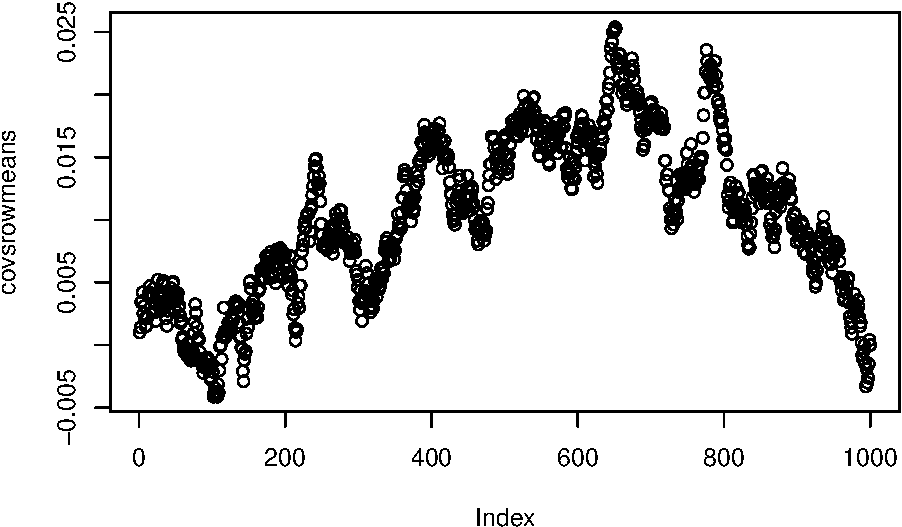
\includegraphics{./figures/unnamed-chunk-10-1.pdf}

\begin{Shaded}
\begin{Highlighting}[]
\NormalTok{corrrowmeans }\OtherTok{\textless{}{-}}\NormalTok{ JuliaCall}\SpecialCharTok{::}\FunctionTok{julia\_eval}\NormalTok{(}\StringTok{"corrrowmeans"}\NormalTok{)}
\FunctionTok{plot}\NormalTok{(corrrowmeans)}
\end{Highlighting}
\end{Shaded}

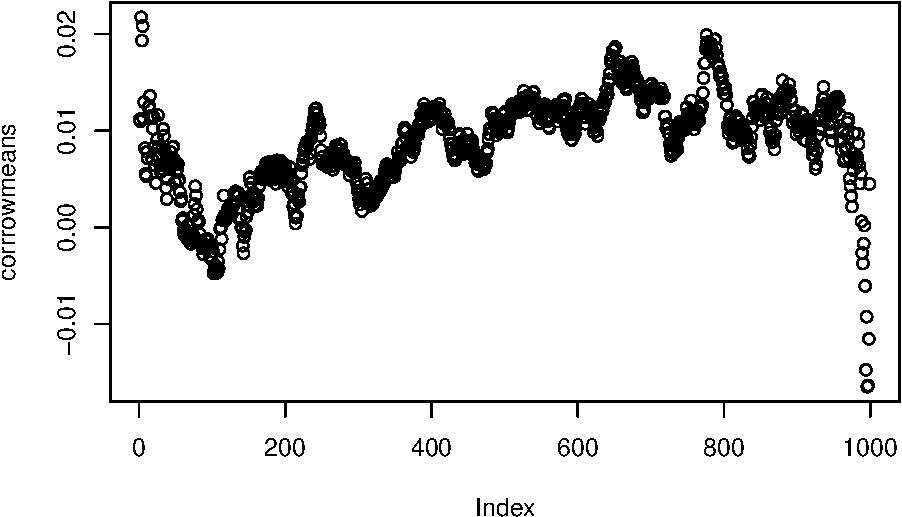
\includegraphics{./figures/unnamed-chunk-10-2.pdf}

\hypertarget{what-information-does-the-sample-covariance-provide}{%
\subsection{What information does the sample covariance
provide?}\label{what-information-does-the-sample-covariance-provide}}

We know that because the Private variable (binary variable) has only 2
possible values, its covariance with other variables is always going to
be relatively small and will not provide much information.

\newpage

\hypertarget{what-information-does-the-sample-correlation-provide}{%
\subsection{What information does the sample correlation
provide?}\label{what-information-does-the-sample-correlation-provide}}

\end{document}
